\chapter{Automatic differentiation}

\section{Introduction: differentiation methods}

Suppose that we have a function $f: \mathbb{R}^n \to \mathbb{R}^m$ that we want to differentiate.
We have many methods to do so:

\begin{enumerate}
    \item \textbf{Manual differentiation}: we can differentiate the function by hand.

    \begin{itemize}
        \item Pros: it is exact, fast, and good for theory
        \item Cons: it is error-prone, time-consuming, and difficult for complex functions
    \end{itemize}

    \item \textbf{Numerical differentiation}: we can approximate the derivative by finite differences.
    
    \begin{itemize}
        \item Pros: it is easy to implement
        \item Cons: it is slow, inaccurate (round-off and truncation errors), and not suitable for complex functions
    \end{itemize}

    Let us look at the example of finite differences in 1 dimension. We can formulate 3 ways to 
    approximate the derivative of a function $f: \mathbb{R} \to \mathbb{R}$ at a point $x$:

    \begin{itemize}
        \item Forward difference: $f'(x) \approx \frac{f(x + h) - f(x)}{h}$
        \item Backward difference: $f'(x) \approx \frac{f(x) - f(x - h)}{h}$
        \item Central difference: $f'(x) \approx \frac{f(x + h) - f(x - h)}{2h}$
    \end{itemize}

    The problem with the Finite Differences method (FDM) is that it presents two types of
    errors:

    \begin{itemize}
        \item \textbf{Truncation error}: it is the error that arises due to the approximation of the derivative.
        It is a consequence of the fact that we are using a Taylor series to approximate the derivative.
        This error decreases as $h$ decreases. For forward and backward differences, the error is $O(h)$, while
        for central differences, the error is $O(h^2)$.

        \item \textbf{Round-off error}: it is the error that arises due to the finite precision of the computer.
        It is a consequence of adding two numbers of different magnitudes, or subtracting two numbers that are 
        close to each other. This error increases as $h$ decreases. 
    \end{itemize}

    The following graph represents the trade-off between the truncation and round-off errors:

    \begin{figure}[H]
        \centering
        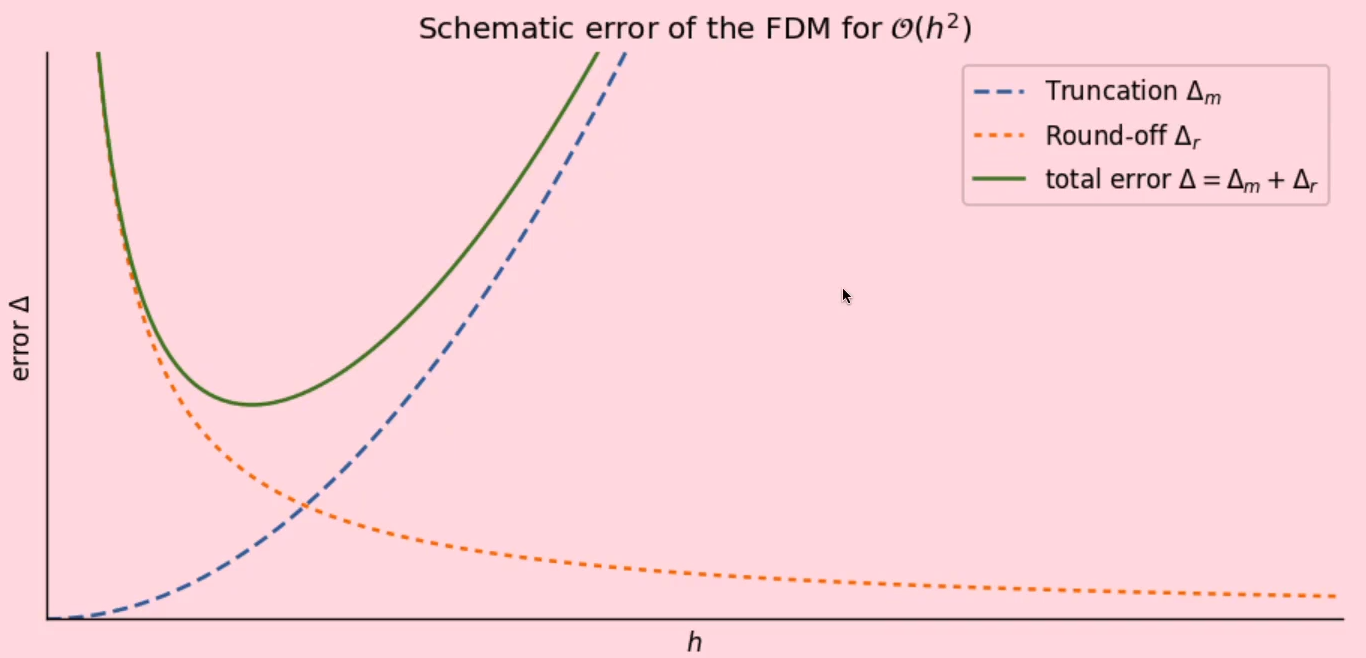
\includegraphics[width=0.6\textwidth]{figures/round-off_vs_trunc.png}
        \caption{Trade-off between truncation and round-off errors}
    \end{figure}

    And we can actually see this in an example:

    \begin{lstlisting}[language=Python]
import numpy as np

def forward_diff(f, x, h):
    return (f(x + h) - f(x)) / h

def centered_diff(f, x, h):
    return (f(x + h) - f(x - h)) / (2 * h)

h = np.logspace(-16, 0, num=500, endpoint=True)
x = 1.0
D1f = forward_diff(np.sin, x, h)
D2f = centered_diff(np.sin, x, h)
err1 = np.abs(D1f - np.cos(x))
err2 = np.abs(D2f - np.cos(x))
\end{lstlisting}

Then, the plot of the errors is:

\begin{figure}[H]
    \centering
    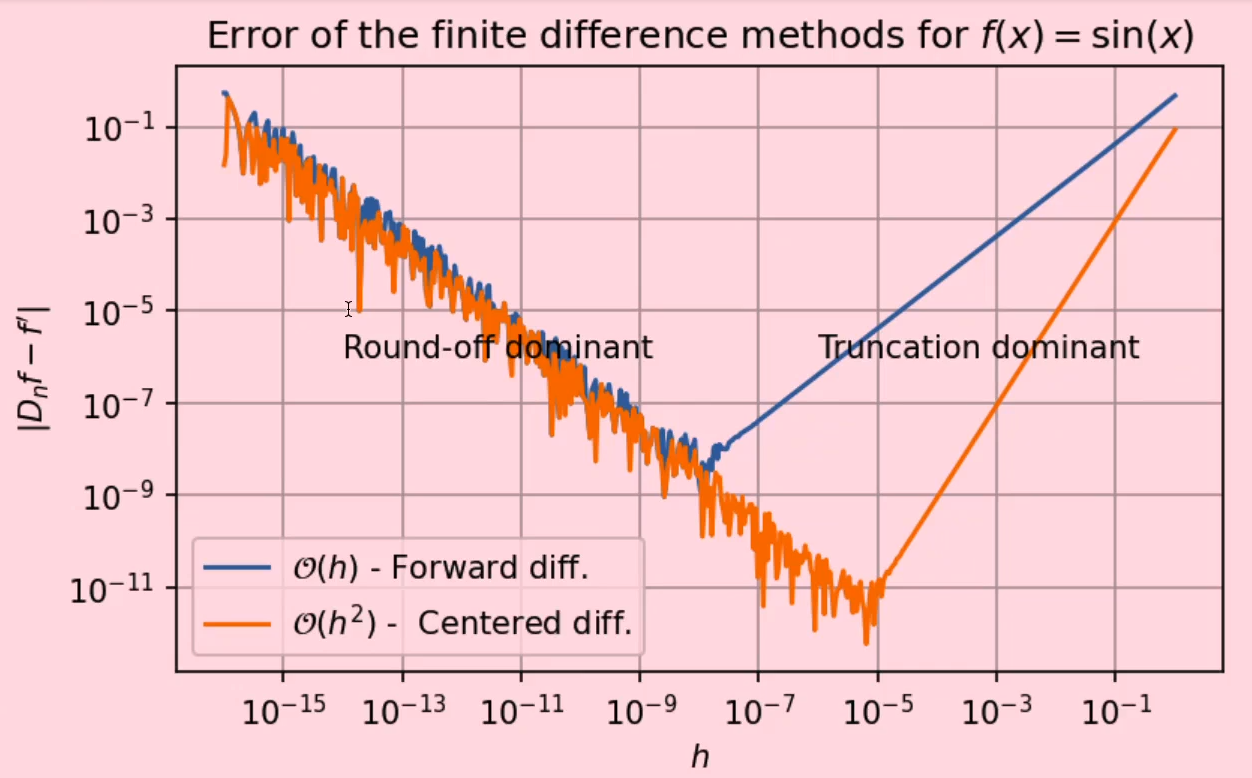
\includegraphics[width=0.6\textwidth]{figures/example_roundoff-trunc.png}
    \caption{Errors of the finite differences method}
\end{figure}

    \item \textbf{Symbolic differentiation}: we can use a computer algebra system (CAS) to compute the derivative symbolically.
    
    \begin{itemize}
        \item Pros: it is exact, good for theory.
        \item Cons: it is slow, memory-intensive, and can cause expression swell for complex functions.
    \end{itemize}

    \item \textbf{Automatic differentiation}: it is a technique that computes the derivative of a function by applying the chain rule.
    
    \begin{itemize}
        \item Pros: it is exact, fast, and general (good for complex functions).
        \item Cons: it is difficult to implement, and it requires a good understanding of the chain rule.
    \end{itemize}

\end{enumerate}

In this chapter, we will focus on automatic differentiation (AD). One of the main methods
of AD is the backward propagation algorithm, which is used in deep learning to compute the gradients
of the loss function with respect to the parameters of the model.\\

Automatic differentiation (AD) is a technique that it is based on the idea
of splitting the computation of the derivative of a function into elementary operations:

\begin{itemize}
    \item Unitary operations
    \item Exponentials, logarithms, trigonometric functions, etc.
\end{itemize}


\section{Wengert list}

Suppose that we have a function $f: \mathbb{R}^n \to \mathbb{R}^m$ that we want to
compute in simple steps. We can represent the function as a sequence of elementary operations
in a Wengert list:

\begin{enumerate}
    \item Define input variables, $v_{i-n} \; \forall i = 1, ..., n$, such that $v_{i-n} = x_i$.
    \item Define intermediate variables, $v_i \; \forall i = n+1, ..., p$, such that $v_i = g_i(v_{j_1}, ..., v_{j_k})$
    for some elementary operation $g_i$.
    \item Define output variables, $y_{i-p} \; \forall i = p+1, ..., m$, such that $y_i = [f(x)]_i$.
\end{enumerate}

For example, consider the function $f(x) = \sin((x_1 + x_2) \cdot x_2^2)$. We can represent
this function as a Wengert list:

\begin{enumerate}
    \item Define input variables: $v_{-1} = x_1$, $v_0 = x_2$.
    \item Define intermediate variables: $v_1 = v_{-1} + v_0$, $v_2 = v_0^2$, $v_3 = v_1 \cdot v_2$, $v_4 = \sin(v_3)$.
    \item Define output variable: $y_1 = v_4$.
\end{enumerate}

The Wengert list can be represented as a computational graph:

\begin{figure}[H]
    \centering
    \resizebox{0.3\textwidth}{!}{%
    \begin{circuitikz}
    \tikzstyle{every node}=[font=\normalsize]
    \draw  (8.5,4.75) circle (0.5cm) node {\normalsize $v_{-1}$} ;
    \draw  (12,4.75) circle (0.5cm) node {\normalsize $v_0$} ;
    \draw  (8.5,7) ellipse (1.5cm and 0.5cm) node {\normalsize $v_1 = v_{-1}+v_0 $} ;
    \draw  (12,7) ellipse (1.5cm and 0.5cm) node {\normalsize $v_2 = v_0^2$} ;
    \draw  (10.25,9.5) ellipse (1.5cm and 0.5cm) node {\normalsize $v_3 = v_1+v_2$} ;
    \draw  (10.25,12.25) ellipse (1.5cm and 0.5cm) node {\normalsize $y_1 = sin(v_3)$} ;
    \draw [->, >=Stealth] (8.5,5.25) -- (8.5,6.5);
    \draw [->, >=Stealth] (12,5.25) -- (12,6.5);
    \draw [->, >=Stealth] (8.5,7.5) -- (9.5,9);
    \draw [->, >=Stealth] (12,7.5) -- (11,9);
    \draw [->, >=Stealth] (11.5,5) -- (9.25,6.5);
    \draw [->, >=Stealth] (10.25,10) -- (10.25,11.75);
    \end{circuitikz}
    }%
    \label{fig:my_label}
    \caption{Computational graph of the Wengert list}
\end{figure}

\section{Forward mode}

The forward mode of automatic differentiation is based on the idea of computing the derivative
of a function by applying the chain rule in the forward direction. The forward mode is useful
when the function has more inputs than outputs, i.e., $n > m$.\\

We can implement the forward mode of automatic differentiation using the Wengert list. 
The algorithm is as follows:

\begin{enumerate}
    \item On the initialization step, we set one of the input variables to 1, and the rest to 0.
    This variable represents which derivative we want to compute.

    \item We calculate the derivatives of the intermediate variables by applying the chain rule.
    
    \item We calculate the derivatives of the output variables by applying the chain rule.
    
    \item We return the derivatives of the output variables.
\end{enumerate}

For example, consider the function $f(x) = \sin((x_1 + x_2) \cdot x_2^2)$. We can compute
the derivative of the function with respect to $x_1$ and $x_2$ using the forward mode of automatic differentiation.
We will use the dot notation to represent the derivative of a variable:

\begin{enumerate}
    \item Set $\dot{v}_{-1} = 1$, $\dot{v}_0 = 0$ (we want to compute the derivative with respect to $x_1$).
    \item Derivate the intermediate variables. 
    
    \begin{itemize}
        \item $\dot{v}_{1} = \dot{v}_{-1} + \dot{v}_0$
        \item $\dot{v}_{2} = 2 \cdot v_0 \cdot \dot{v}_0$
        \item $\dot{v}_{3} = \dot{v}_1 \cdot v_2 + v_1 \cdot \dot{v}_2$
        \item $\dot{v}_{4} = \cos(v_3) \cdot \dot{v}_3$
    \end{itemize}

    \item Return $\dot{y}_1 = \dot{v}_4$.

\end{enumerate}

Notice that to compute the derivative of the function with respect to $x_1$ and $x_2$, we need to
compute the intermediate variables for a certain point $x$ (because we have to use the values of the variables
to compute the derivatives). This method of differentiation does not return a symbolic 
expression for the derivative, but the value of the derivative at a certain point.\\

Note that this method is not efficient when the function has more inputs than outputs, i.e., $m << n$.
This is because we have to do the forward pass for each input variable, which can be computationally expensive.

\section{Dual numbers}

We define a dual number as a pair of real numbers $(a, b)$, where $a$ is the real part, and $b$ is the dual part.
It is expressed as follows:

\begin{equation}
    z = a + b \varepsilon
\end{equation}

where $\varepsilon$ is a number such that $\varepsilon \neq 0 \; \wedge \; \varepsilon^2 = 0$. 
We can define the operations of addition and multiplication as follows:

\begin{itemize}
    \item Addition: 
    $$(a + b \varepsilon) + (c + d \varepsilon) = (a + c) + (b + d) \varepsilon$$

    \item Multiplication: 
   $$(a + b \varepsilon) \cdot (c + d \varepsilon) = ac + (ad + bc) \varepsilon$$

\end{itemize}

Now, let us consider a generic function $f(\cdot)$. We will evaluate the function in a 
dual number $z = x + \varepsilon$. We can expand the function in a Taylor series around $x$:

\begin{equation}
    f(z) = f(x + \varepsilon) = f(x) + f'(x) \varepsilon + O(\varepsilon^2)
\end{equation}

Because $\varepsilon^2 = 0$, we have that:

\begin{equation}
    f(z) = f(x) + f'(x) \varepsilon
\end{equation}

This means that the dual part of the function evaluated in a dual number is the derivative of the function
evaluated at the real part of the dual number. This is the key idea behind the dual numbers: we can use them
to compute the derivative of a function by evaluating the function in a dual number.\\

Let us expand the idea to a general dual number $a + b \varepsilon$. We can evaluate the function $f(\cdot)$
in the dual number as follows:

\begin{equation}
    f(a + b \varepsilon) = f(a) + f'(a) b \varepsilon
\end{equation}

With this property, we can also compute the derivative of a composite function. Suppose that we 
have two functions $f(\cdot)$ and $g(\cdot)$. We can compute the derivative of the composite 
function $h(\cdot) = f(g(\cdot))$ as follows:

\begin{equation}
    h(x + \varepsilon) = f(g(x + \varepsilon)) = f(g(x) + g'(x) \varepsilon) = f(g(x)) + f'(g(x)) g'(x) \varepsilon
\end{equation}

This means that we can compute the derivative of a composite function by evaluating the functions 
in dual numbers.\\

We can also redefine the dual numbers to obtain the second derivative of a function. We just need to
define $\varepsilon^2 \neq 0$ and $\varepsilon^3 = 0$. 
